\documentclass[]{jarticle}          % 一段組
%\documentclass[twocolumn]{jarticle} % 二段組

\textwidth 180mm
\textheight 255mm
\oddsidemargin -12mm
\topmargin -15mm
\columnsep 10mm

%\vspace{0.5cm} % 一段組の場合はコメントアウトした方が体裁がよいx
%] % 一段組の場合はコメントアウトする

\usepackage{styles/labheadings}
\usepackage[dvipdfmx]{graphicx,color}
\usepackage{amsmath,amssymb}
\usepackage{url}
% 追加
\usepackage[hang,small,bf]{caption}
\usepackage[subrefformat=parens]{subcaption}
\usepackage{float}
\captionsetup{compatibility=false}

\input{numerical_definition.tex}
% report.texと同じディレクトリにnumerical_definition.texを入れておけば上の書き方でもいいはずです

\usepackage[
  dvipdfm,
  bookmarks=true,
  bookmarksnumbered=true,
  colorlinks=true]{hyperref}
\AtBeginDvi{\special{pdf:tounicode EUC-UCS2}}

\pagestyle{labheadings}
\headerleft{2次元フロアマップからのシーンの3次元モデルの作成}   % ヘッダの左側のタイトル
\headerright{2024年10月10日}  % ヘッダの右側のタイトル

\begin{document}

%\twocolumn % 一段組の場合はコメントアウトする

\vspace*{2ex}
\begin{center}
 {\Large \bf 全方位画像を用いた三次元モデルのテクスチャ取得}\\ % タイトル
 \vspace*{5mm}
 {\large M1 田川幸汰}% 発表者名
\end{center}

%\vspace{0.5cm} % 一段組の場合はコメントアウトした方が体裁がよいx
%] % 一段組の場合はコメントアウトする

%新しく作成したコマンド
% \newcommand{\reffig}[1]{\hyperref[#1]{図\ref{#1}}}
% \newcommand{\refeq}[1]{\hyperref[#1]{式(\ref{#1})}}
% \newcommand{\reftab}[1]{\hyperref[#1]{表\ref{#1}}}
% \newcommand{\refsec}[1]{\hyperref[#1]{\ref{#1}章}}
% \newcommand{\refsubsec}[1]{\hyperref[#1]{\ref{#1}節}}

% 数式
%\begin{equation}
%  数式記述  
%  \label{ラベル名}
%\end{equation}

% 図
% \begin{figure}[!ht]
%   \begin{center}
%     \includegraphics[scale=0.5]{figures/画像ファイル名}
%     \caption{キャプション名}
%     \label{ラベル名}
%   \end{center}
% \end{figure}

% リスト
% \begin{enumerate or itemize}
%   \item 
% \end{enumerate or itemize}
\section{概要}
カメラ姿勢推定の方法と全方位画像の枚数を変えた際のテクスチャ画像と、
実際にテクスチャを割り当てた3次元モデルを示す。
そこから、現状の課題と、今後の研究方針について報告する。

\section{進捗}
\subsection{カメラパラメータ手動入力し、全方位画像1枚使用}
全方位カメラのパラメータである回転行列、並進ベクトルを手動で入力し、全方位画像を1枚テクスチャとして使用した
場合のテクスチャ画像の一部を\hyperref[one]{図\ref{one}}に示す

\begin{figure}[H]
  \begin{center}
    \begin{tabular}{cc}
      \includegraphics[keepaspectratio, scale=0.1]{figures/texture1/texture/texture_1_0.png}&
      \includegraphics[keepaspectratio, scale=0.1]{figures/texture1/texture/texture_1_16.png}\\
      \includegraphics[keepaspectratio, scale=0.1]{figures/texture1/texture/texture_1_21.png}&
      \includegraphics[keepaspectratio, scale=0.1]{figures/texture1/texture/texture_1_1.png}\\
    \end{tabular}
  \end{center}
  \caption{テクスチャ画像(1)}
  \label{one}
\end{figure}

これらを用いて生成された3次元モデルを\hyperref[two]{図\ref{two}}に示す。テクスチャ間の歪は小さく、比較的ずれも小さく再現することができているが、テクスチャを取得できていない面が多く残っている。

\begin{figure}[H]
  \begin{center}
    \begin{tabular}{c}
      \includegraphics[keepaspectratio, scale=0.3]{figures/C5F1.png}
    \end{tabular}
  \end{center}
  \caption{3次元モデル(1)}
  \label{two}
\end{figure}

\subsection{カメラパラメータ手動入力し、全方位画像複数枚使用}
全方位カメラのパラメータである回転行列、並進ベクトルを手動で入力し、全方位画像を3枚テクスチャとして使用した
場合のテクスチャ画像の一部を\hyperref[three]{図\ref{three}}に示す

\begin{figure}[H]
  \begin{center}
    \begin{tabular}{cc}
      \includegraphics[keepaspectratio, scale=0.1]{figures/texture2/texture/texture_0_3.png}&
      \includegraphics[keepaspectratio, scale=0.1]{figures/texture2/texture/texture_0_15.png}\\
      \includegraphics[keepaspectratio, scale=0.1]{figures/texture2/texture/texture_2_2.png}&
      \includegraphics[keepaspectratio, scale=0.1]{figures/texture2/texture/texture_2_17.png}\\
    \end{tabular}
  \end{center}
  \caption{テクスチャ画像(2)}
  \label{three}
\end{figure}

これらを用いて生成された3次元モデルを\hyperref[four]{図\ref{four}}に示す。テクスチャ間の歪が大きくなっているが、全ての面でテクスチャを取得できている。

\begin{figure}[H]
  \begin{center}
    \begin{tabular}{c}
      \includegraphics[keepaspectratio, scale=0.3]{figures/C5F2.png}
    \end{tabular}
  \end{center}
  \caption{3次元モデル(2)}
  \label{four}
\end{figure}



\subsection{カメラパラメータ推定、全方位画像複数枚使用}
全方位カメラのパラメータである回転行列、並進ベクトルを2次元座標と3次元座標の対応から推定し、全方位画像を1枚テクスチャとして使用した
場合のテクスチャ画像の一部を\hyperref[five]{図\ref{five}}に示す

\begin{figure}[H]
  \begin{center}
    \begin{tabular}{cc}
      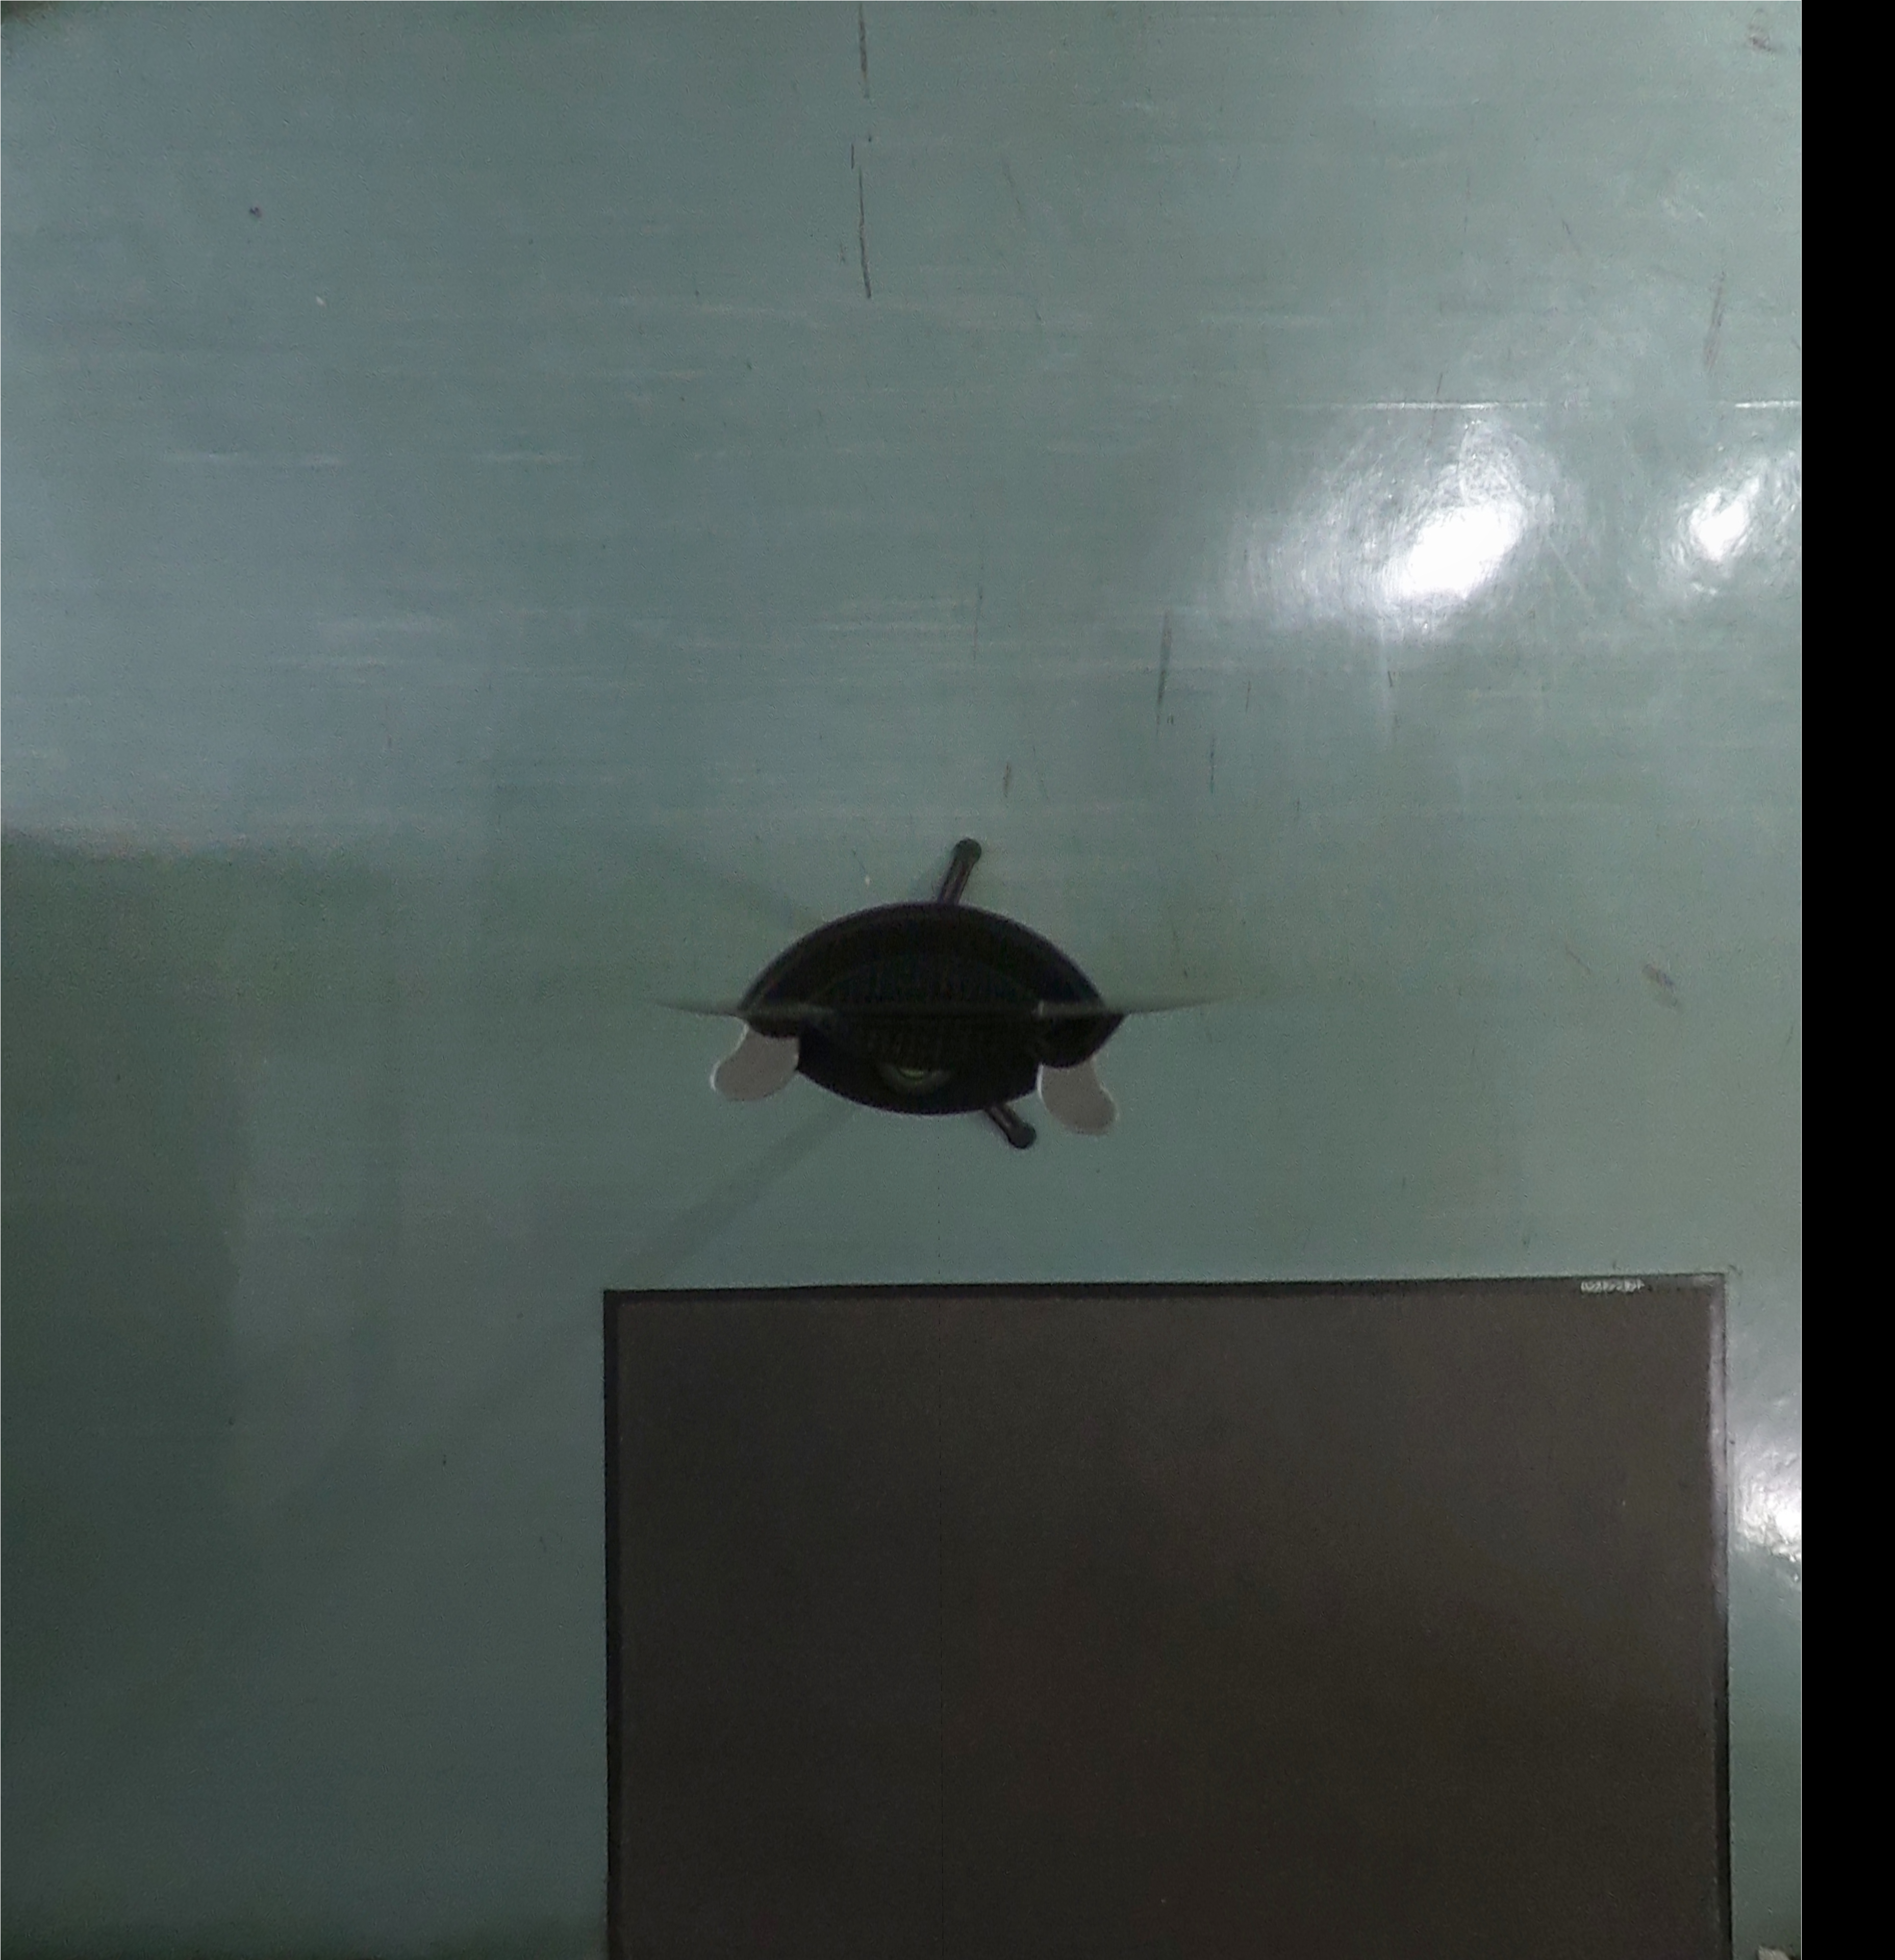
\includegraphics[keepaspectratio, scale=0.1]{figures/texture3/texture/texture_0_0.png}&
      \includegraphics[keepaspectratio, scale=0.1]{figures/texture3/texture/texture_0_5.png}\\
    \end{tabular}
  \end{center}
  \caption{テクスチャ画像(3)}
  \label{five}
\end{figure}

明らかにテクスチャが正しく取得することができていない。なお、同様のプログラムを用いてシミュレーション上では正しいカメラパラメータを推定することができているため、
プログラムを移行する際に何らかの問題が発生してしまっていることが予想される。

これらを用いて生成された3次元モデルを\hyperref[four]{図\ref{six}}に示す。白がカメラの大凡の位置であるが、そこから大きくずれてしまっている。

\begin{figure}[H]
  \begin{center}
    \begin{tabular}{c}
      \includegraphics[keepaspectratio, scale=0.3]{figures/C5F3.png}
    \end{tabular}
  \end{center}
  \caption{3次元モデル(2)}
  \label{six}
\end{figure}

\subsection{今後の目標}
まずは複数の線方位画像を用いる場合のプログラムが間違えていないか確認する必要がある。プログラムに問題がない場合、
テクスチャ画像間のずれを小さくするにはどうすればいいか、カメラ位置姿勢推定の精度を向上させる以外のアプローチを考える。

次に、カメラパラメータの推定を正しく行う必要がある。これについてもプログラムのミスを早急に改善し、
3次元モデルがどのように表示されるか確かめる。
\end{document}
